\begin{figure*}[t] \centering
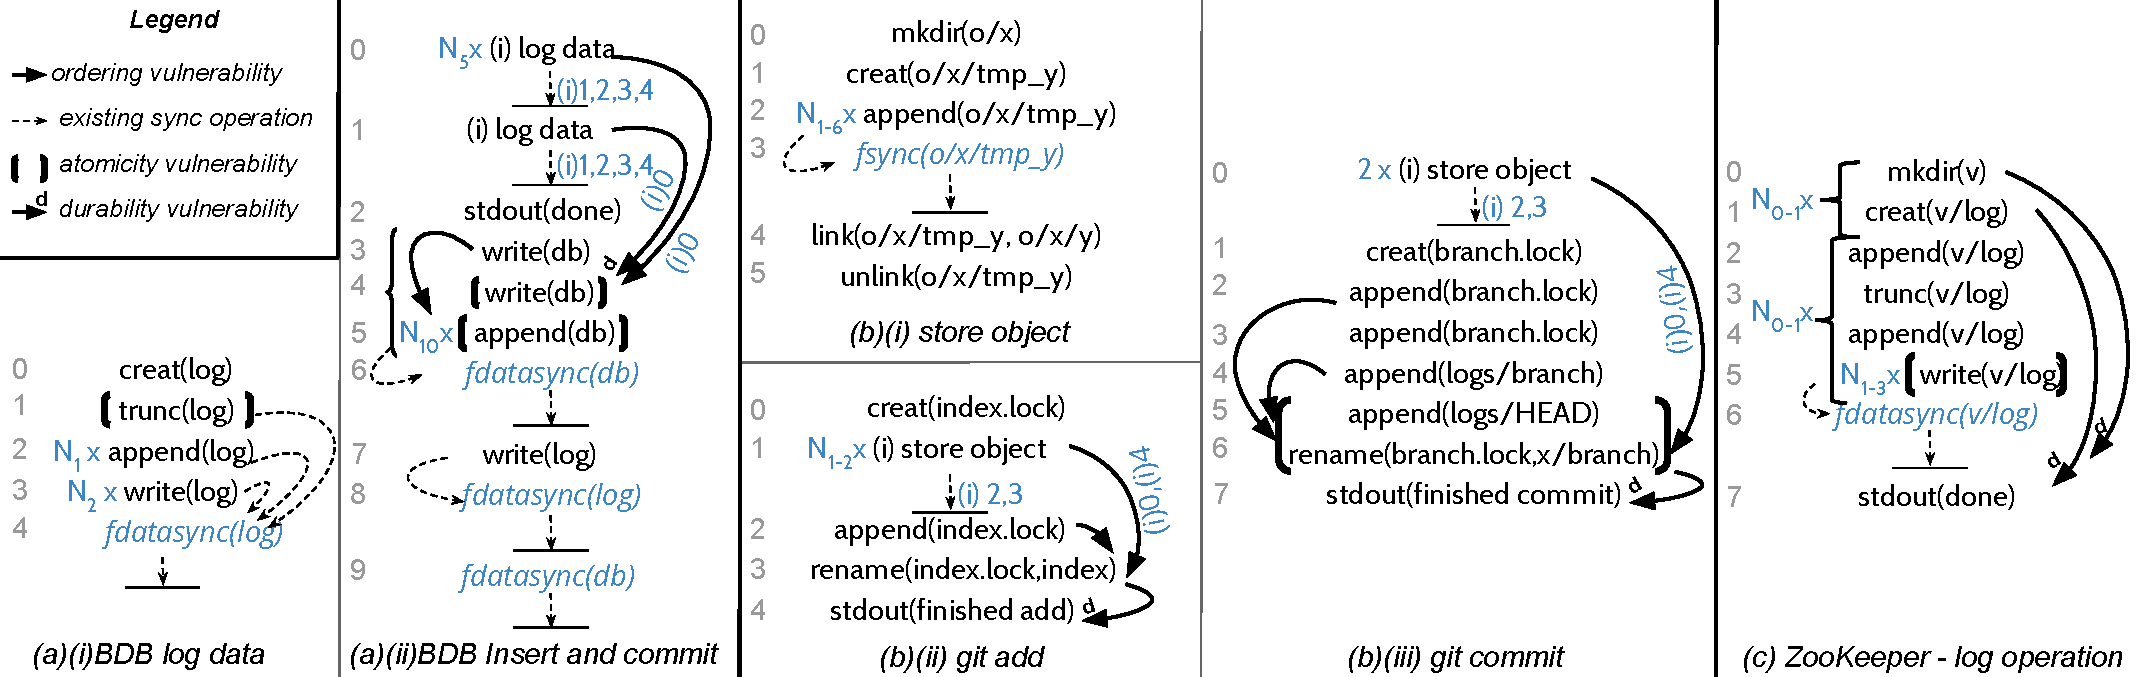
\includegraphics[width=\textwidth]{figs/prot-combined.pdf}
\caption{\label{fig-prot}\textbf{Protocol Diagrams.} {\footnotesize\textit{
(a), (b), and (c) show the modularized update protocol for Git, ZooKeeper, and
BerkeleyDB-BTree respectively. Repeated operations in a protocol
are shown next to each operation, and if the number of repetitions can vary,
the variation is specified. Ordering dependencies are indicated with arrows,
and dependencies between modules are indicated by the numbers on the arrows,
corresponding to line numbers in modules. Dotted, vertical arrows ending at a horizontal
line represent ordering dependencies already enforced using sync operations in the
application. Dark, bold arrows represent new ordering dependencies
discovered; \textbf{d} on the arrow represents a durability requirement.
Operations inside dark brackets must be persisted together atomically.
}}}
\end{figure*}
\newcommand{\refprotbdb}{\ref{fig-prot}(a)}
\newcommand{\refprotgit}{\ref{fig-prot}(b)}
\newcommand{\refprotzookeeper}{\ref{fig-prot}(c)}

